\chapter{Machine Comprehension}
\label{chap:comprehension}
In this chapter a brief introduction to the machine comprehension task is given, followed by the definition and application of our metric, that was defined for measuring similarity between concept graphs. After our baseline for the task presented.

The 2018 Semeval Task \textit{Machine comprehension using commonsense
	knowledge}\footnote{\url{https://competitions.codalab.org/competitions/17184}}
requires participants to train systems that can choose the
correct answer to simple multiple choice questions based on short
passages describing simple chains of events. Data for both training and
testing is extracted from the \texttt{MCScript} dataset
\cite{Ostermann:2018}. Some questions can only be
answered using commonsense knowledge, and are
explicitly labeled as such. For example, one passage might describe a
story of a gardener planting a tree, and one of the questions would
subsequently ask whether the gardener used his hands or a shovel to dig
a hole for the tree, even though the answer to this question is not
present in the passage. The top two systems, \texttt{HFL-RC}
\cite{Chen:2018} and
\texttt{Yuanfudao} \cite{Wang:2018} achieved accuracy scores of
$84.15\%$ and $83.95\%$ on the test data, respectively. In our experiments we used
semantic graphs to augment the \texttt{Yuanfudao} system, since its source
code is publicly
available\footnote{\url{https://github.com/intfloat/commonsense-rc}} and since it already employs successfully a
knowledge base representing semantic relationships among pairs of words.

\subsection{Comprehension, entailment, and knowledge bases}

In the next section we shall present a simple method for measuring
\textit{support}, the continuous counterpart of \textit{entailment},
based on graphical representations of meaning, and use this metric in a
baseline for machine comprehension and to improve a state of the art
MC system.
Although explicit representations of semantics are rarely used for this purpose,
in recent years there have been several attempts at leveraging lexical
ontologies in machine comprehension, and the approach of using textual
entailment as an intermediary task is also not new. \cite{Wang:2016}
achieves competitive results on the \texttt{MCTest} dataset
\cite{Richardson:2013} by generating
answer candidates and ranking them using a separate RTE system, which is
trained on the Stanford Natural Language Inference (SNLI) dataset
\cite{Bowman:2015}
but also relies on an explicit measure of lexical overlap between sentence
pairs. Other recent systems are various extensions of a baseline
proposed by \cite{Richardson:2013} that measures a weighted overlap
between pairs of bag-of-words representations, e.g. \cite{Wang:2015b}
applies the frame
semantic parser of \cite{Das:2010} and includes features representing
overlap between bag-of-frame and bag-of-argument representations.
Finally, the \texttt{Yuanfudao} system presented in this section is the most
recent example of enhancing the performance of an MC system using a lexical
knowledge base: ablation studies show that their top-ranking accuracy score of
$83.84\%$ drops to $82.78\%$ if \texttt{ConceptNet}-based features are removed.

\section{Method}
\label{sec:method}

We define a simple metric between pairs of \texttt{4lang} graphs that
we intend to use for measuring entailment between a paragraph and a
sentence. We shall define the degree to which some graph $G_1$
\textit{supports} another graph $G_2$ as the ratio of edges in $G_2$
that are also present in $G_1$:

\[ S(G_1, G_2) =\frac{|E(G_1)\cap E(G_2)|}{|E(G_2)|}\]

Two (directed) edges are identical if their source
and target nodes and their labels are all identical. Based on early
findings we used only \textit{expanded} \texttt{4lang} graphs (see
Section~\ref{sec:4lang}) for measuring support. 
To create a simple baseline solution for the Machine Comprehension task,
we compare answer candidates to each question by comparing the degree of
support for each in the passage, based on the \texttt{4lang} representations of
each piece of text. For wh-questions we can create representations of
each answer by merging the question graph's wh-node with the graph of
each answer graph (see Figure~\ref{fig:merge}), for this we use the \textbf{/rally} endpoint of our service defined in the previous chapter. Our baseline method will simply
pick the answer candidate with the higher support score.

\begin{figure}
	\centering
	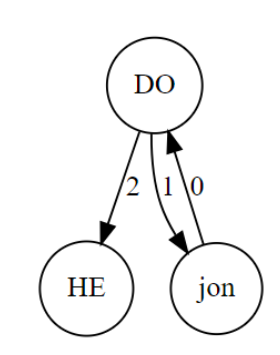
\includegraphics[scale=0.4]{figures/merge}
	\caption{Merged graph of answer candidate \textit{"Jon"} for the
		question \textit{Who did it?}}
	\label{fig:merge}
\end{figure}

\subsection{Experiments}
\label{sec:exp}

Demonstrating the algorithm behind our baseline, let's look at the example passage:
\begin{center}
	\textit{ "I went into my bedroom and flipped the light switch. Oh, I see that the ceiling lamp is not turning on. It must be that the light bulb needs replacement. I go through my closet and find a new light bulb that will fit this lamp and place it in my pocket. I also get my stepladder and place it under the lamp. I make sure the light switch is in the off position. I climb up the ladder and unscrew the old light bulb. I place the old bulb in my pocket and take out the new one. I then screw in the new bulb. I climb down the stepladder and place it back into the closet. I then throw out the old bulb into the recycling bin. I go back to my bedroom and turn on the light switch. I am happy to see that there is again light in my room."}
\end{center}
And a question related to the text: \textit{Which room did the light go out in?} and the answers:
\begin{itemize}
	\item \textit{"Kitchen."}
	\item \textit{"Bedroom."}
\end{itemize}
First we build the expanded graph from the text. After we build the merged graphs (for the demonstration, we now only build the graphs without expansion) seen in Figure \ref{fig:merge1} and Figure \ref{fig:merge2}. The graph without merging can be seen in Figure \ref{fig:merge3}. After the merging, we compare both of the graphs to the passage graph applying our defined metric.

\begin{figure}
	\centering
	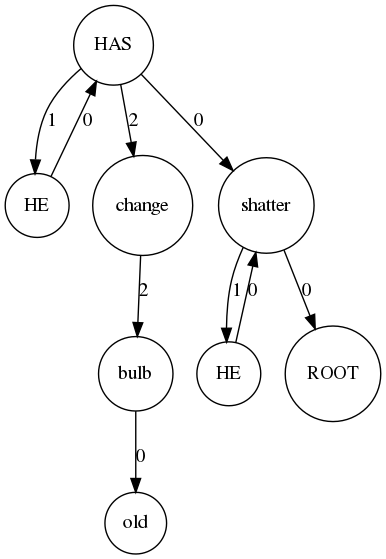
\includegraphics[scale=0.4]{figures/comp}
	\caption{Merged graph of answer candidate \textit{"Kitchen."}}
	\label{fig:merge1}
\end{figure}

\begin{figure}
	\centering
	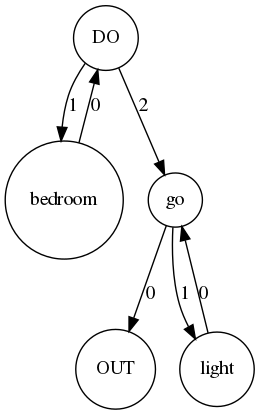
\includegraphics[scale=0.4]{figures/comp2}
	\caption{Merged graph of answer candidate \textit{"Bedroom."}}
	\label{fig:merge2}
\end{figure}

\begin{figure}
	\centering
	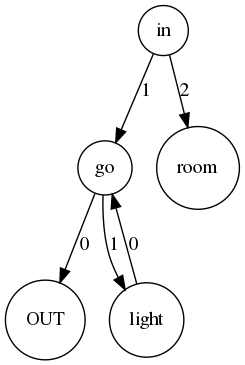
\includegraphics[scale=0.4]{figures/compdef}
	\caption{Graph built from the question}
	\label{fig:merge3}
\end{figure}

We tested the baseline method described in the previous section on a
subset of all questions in the train section of the MC dataset:
wh-questions that were not
categorized as "common-sense". Of this subset of 5,375 questions (of a
total of 9,731), our
method correctly answers 3,671, achieving an accuracy score of $68.3\%$.
We then proceeded to use the metric underlying our baseline as an
additional feature in the \texttt{Yuanfudao} system. 

In the next chapter we will briefly give an introduction into the field of deep learning in general, and particularly in NLP applications, and then we will demonstrate the Yuanfudao system.